\documentclass{beamer}

\usetheme{Hannover}

\title{Presentación del primer proyecto de programación}
\author{Ariadna Velázquez Rey}
\date{\today}

\usepackage{graphicx}
\graphicspath{{../}}

\begin{document}

\begin{frame}
    \maketitle

    \begin{figure}[h]
        \centering
        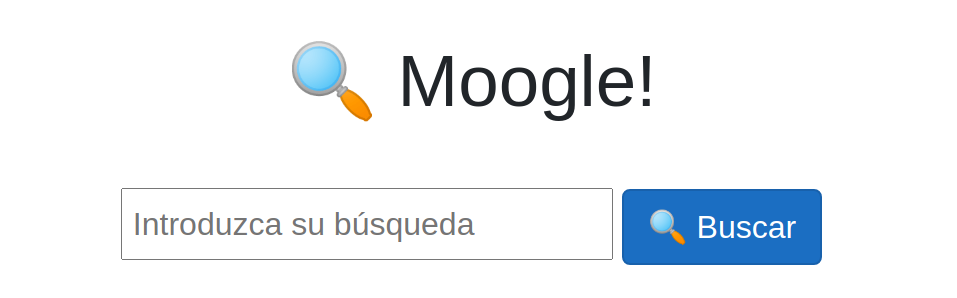
\includegraphics[width=1\textwidth]{moogle}
    \end{figure}
\end{frame}

\begin{frame}
    \frametitle{Introducción}
    Esta es mi versión del Moogle, el objetivo de este proyecto es encontrar los documentos que contienen las palabras 
    de la búsqueda del usuario. 

    El método empleado por el motor de búsqueda es la creación de matrices de datos para la comparación y cálculo de 
    estos valores, de tal manera que con el resultado se determine la relevancia de cada documento con respecto a la 
    frase proporcionada por el usuario.
\end{frame}

\begin{frame}
    \frametitle{Generalidades}
      El proyecto presenta varios procesos para su correcto funcionamiento y mayor eficiencia:

    \begin{itemize}
        \item El score no aparece al devolver los textos, sin embargo es el encargado del orden de relevancia en el 
        que se presentan los documentos, que se muestran organizados descendentemente de acuerdo a este valor.
        \item El snippet es un fragmento de texto, del documento relevante, en el que aparece la frase de la búsqueda 
        o un fragmento de esta.
    \end{itemize}    
\end{frame}

\begin{frame}
    \frametitle{Generalidades}
    \begin{itemize}
        \item Cuenta con los operadores de inclusión (\^{}) y exclusión (!) que determinan si el documento puede ser 
        devuelto. En el primer caso si la palabra que inicie con el char especificado no está incluida este pierde 
        toda su relevancia; en el segundo caso ocurre lo contrario, si la palabra aparece este se excluye de la lista.
        \item En el caso del operador de relevancia (*) su función es aumentar la importancia asignada a la palabra 
        durante la formación de las matrices del motor de búsqueda, lo que influye en el score de los documentos.
    \end{itemize}

    Además, contiene un script de bash que permite ejecutar el proyecto, añadir documentos .txt a /Content, generar y 
    mostrar el informe y la presentación .tex, así como eliminar archivos secundarios innecesarios.
\end{frame}


\begin{frame}
    \frametitle{Especificaciones}
    Dentro del motor de búsqueda se realizan múltiples procesos que en conjunto permiten el funcionamiento del moogle.
    El código del proyecto está dividido en clases dependiendo de su objetivo. 
    
    La más básica es en la que se encuentran los métodos auxiliares para analizar los textos que es la 
    \textbf{Class Obtein}. El comando \textit{Regex("[\^{}a-zA-Z0-9 ]")}, y las ligeras variaciones que se le hacen, 
    es uno de los más utilizados pues elimina los símbolos y chars que puedan afectar a la búsqueda. También contiene 
    el método matemático exacto de la similitud de cosenos. 
\end{frame}

\begin{frame} 
    \frametitle{Especificaciones}
    La \textbf{Class TextAnalize} es la encargada de formar las matrices que permiten la comparación de los documentos
    con el query y su procesamiento para obtener el resultado final. Se realizan los cálculos del TF e IDF (cuyas 
    fórmulas son exactas), se procesan los operadores, el score y el snippet.

    A la \textbf{Class Moogle} solo se le añaden unas pocas líneas de código que llaman a los métodos de 
    \textit{TextAnalize} para organizar el listado final de documentos a devolver en la interfaz gráfica.
\end{frame}

\begin{frame}
    \frametitle{Especificaciones}
    El proyecto cuenta con dos clases que no se emplean en ningún proceso, pero cuyos principios son 
    fundamentales para las operaciones realizadas. Estas son la \textbf{Class Matrix} y  la \textbf{Class Vec},  que 
    están formadas por los cálculos que se pueden hacer algebraicamente con matrices y vectores.

    También presenta un script que se ejecuta con argumentos en la línea de comando y/o con un bucle infinito que 
    muestra una lista con las opciones válidas y solo se detiene con el comando crash, en lugar del común control c; 
    tiene la posibilidad de seleccionar el visualizador de pdf deseado y agregar de manera dinámica documentos .txt a 
    /Content para ejecutarlos en el proyecto.
\end{frame}

\begin{frame}
    \frametitle{Conclusiones}
    En el proceso para realizar este proyecto he puesto en práctica y comprendido el funcionamiento de una de las 
    operaciones más importante en el desarrollo de programas, que es el trabajo con matrices. 
    
    A lo largo de su evolución se han modificado los tipos de variables y los métodos utilizados, hasta encontrar no 
    solo los más sencillos de comprender, sino los más óptimos en cuanto al tiempo de ejecución.

    Sin embargo, lo realmente importante y la mayor huella que deja el moogle al ser el primer proyecto de programación 
    realizado, es el entendimiento de cuán importante es la persistencia, la distribución del tiempo de trabajo y el 
    estar siempre dispuestos a buscar nuevas vías de solución a cualquier desafío computacional que se enfrente.
\end{frame}

\end{document}